% Template for PLoS
% Version 3.4 January 2017
%
% % % % % % % % % % % % % % % % % % % % % %
%
% -- IMPORTANT NOTE
%
% This template contains comments intended
% to minimize problems and delays during our production
% process. Please follow the template instructions
% whenever possible.
%
% % % % % % % % % % % % % % % % % % % % % % %
%
% Once your paper is accepted for publication,
% PLEASE REMOVE ALL TRACKED CHANGES in this file
% and leave only the final text of your manuscript.
% PLOS recommends the use of latexdiff to track changes during review, as this will help to maintain a clean tex file.
% Visit https://www.ctan.org/pkg/latexdiff?lang=en for info or contact us at latex@plos.org.
%
%
% There are no restrictions on package use within the LaTeX files except that
% no packages listed in the template may be deleted.
%
% Please do not include colors or graphics in the text.
%
% The manuscript LaTeX source should be contained within a single file (do not use \input, \externaldocument, or similar commands).
%
% % % % % % % % % % % % % % % % % % % % % % %
%
% -- FIGURES AND TABLES
%
% Please include tables/figure captions directly after the paragraph where they are first cited in the text.
%
% DO NOT INCLUDE GRAPHICS IN YOUR MANUSCRIPT
% - Figures should be uploaded separately from your manuscript file.
% - Figures generated using LaTeX should be extracted and removed from the PDF before submission.
% - Figures containing multiple panels/subfigures must be combined into one image file before submission.
% For figure citations, please use "Fig" instead of "Figure".
% See http://journals.plos.org/plosone/s/figures for PLOS figure guidelines.
%
% Tables should be cell-based and may not contain:
% - spacing/line breaks within cells to alter layout or alignment
% - do not nest tabular environments (no tabular environments within tabular environments)
% - no graphics or colored text (cell background color/shading OK)
% See http://journals.plos.org/plosone/s/tables for table guidelines.
%
% For tables that exceed the width of the text column, use the adjustwidth environment as illustrated in the example table in text below.
%
% % % % % % % % % % % % % % % % % % % % % % % %
%
% -- EQUATIONS, MATH SYMBOLS, SUBSCRIPTS, AND SUPERSCRIPTS
%
% IMPORTANT
% Below are a few tips to help format your equations and other special characters according to our specifications. For more tips to help reduce the possibility of formatting errors during conversion, please see our LaTeX guidelines at http://journals.plos.org/plosone/s/latex
%
% For inline equations, please be sure to include all portions of an equation in the math environment.  For example, x$^2$ is incorrect; this should be formatted as $x^2$ (or $\mathrm{x}^2$ if the romanized font is desired).
%
% Do not include text that is not math in the math environment. For example, CO2 should be written as CO\textsubscript{2} instead of CO$_2$.
%
% Please add line breaks to long display equations when possible in order to fit size of the column.
%
% For inline equations, please do not include punctuation (commas, etc) within the math environment unless this is part of the equation.
%
% When adding superscript or subscripts outside of brackets/braces, please group using {}.  For example, change "[U(D,E,\gamma)]^2" to "{[U(D,E,\gamma)]}^2".
%
% Do not use \cal for caligraphic font.  Instead, use \mathcal{}
%
% % % % % % % % % % % % % % % % % % % % % % % %
%
% Please contact latex@plos.org with any questions.
%
% % % % % % % % % % % % % % % % % % % % % % % %

\documentclass[10pt,letterpaper]{article}
\usepackage[top=0.85in,left=2.75in,footskip=0.75in]{geometry}

% amsmath and amssymb packages, useful for mathematical formulas and symbols
\usepackage{amsmath,amssymb}

% Use adjustwidth environment to exceed column width (see example table in text)
\usepackage{changepage}

% Use Unicode characters when possible
\usepackage[utf8x]{inputenc}

% textcomp package and marvosym package for additional characters
\usepackage{textcomp,marvosym}

% cite package, to clean up citations in the main text. Do not remove.
\usepackage{cite}

% Use nameref to cite supporting information files (see Supporting Information section for more info)
\usepackage{nameref,hyperref}

% line numbers
\usepackage[right]{lineno}

% ligatures disabled
\usepackage{microtype}
\DisableLigatures[f]{encoding = *, family = * }

% color can be used to apply background shading to table cells only
\usepackage[table]{xcolor}

% array package and thick rules for tables
\usepackage{array}

% create "+" rule type for thick vertical lines
\newcolumntype{+}{!{\vrule width 2pt}}

% create \thickcline for thick horizontal lines of variable length
\newlength\savedwidth
\newcommand\thickcline[1]{%
  \noalign{\global\savedwidth\arrayrulewidth\global\arrayrulewidth 2pt}%
  \cline{#1}%
  \noalign{\vskip\arrayrulewidth}%
  \noalign{\global\arrayrulewidth\savedwidth}%
}

% \thickhline command for thick horizontal lines that span the table
\newcommand\thickhline{\noalign{\global\savedwidth\arrayrulewidth\global\arrayrulewidth 2pt}%
\hline
\noalign{\global\arrayrulewidth\savedwidth}}


% Remove comment for double spacing
%\usepackage{setspace}
%\doublespacing

% Text layout
\raggedright
\setlength{\parindent}{0.5cm}
\textwidth 5.25in
\textheight 8.75in

% Bold the 'Figure #' in the caption and separate it from the title/caption with a period
% Captions will be left justified
\usepackage[aboveskip=1pt,labelfont=bf,labelsep=period,justification=raggedright,singlelinecheck=off]{caption}
\renewcommand{\figurename}{Fig}

% Use the PLoS provided BiBTeX style
\bibliographystyle{plos2015}

% Remove brackets from numbering in List of References
\makeatletter
\renewcommand{\@biblabel}[1]{\quad#1.}
\makeatother

% Leave date blank
\date{}

% Header and Footer with logo
\usepackage{lastpage,fancyhdr,graphicx}
\usepackage{epstopdf}
\pagestyle{myheadings}
\pagestyle{fancy}
\fancyhf{}
\setlength{\headheight}{27.023pt}
\lhead{
\includegraphics[width=2.0in]{PLOS-submission.eps}}
\rfoot{\thepage/\pageref{LastPage}}
\renewcommand{\footrule}{\hrule height 2pt \vspace{2mm}}
\fancyheadoffset[L]{2.25in}
\fancyfootoffset[L]{2.25in}
\lfoot{\sf PLOS}

%% Include all macros below

% \newcommand{\lorem}{{\bf LOREM}}
% \newcommand{\ipsum}{{\bf IPSUM}}
\newcommand{\rulemajor}[1]{\section{#1}}

%% END MACROS SECTION


\begin{document}
\vspace*{0.2in}

% Title must be 250 characters or less.
\begin{flushleft}
{\Large
\textbf\newline{Ten simple rules for collaborative lesson development} % Please use "sentence case" for title and headings (capitalize only the first word in a title (or heading), the first word in a subtitle (or subheading), and any proper nouns).
}
\newline
% Insert author names, affiliations and corresponding author email (do not include titles, positions, or degrees).
\\
{Gabriel~A.~Devenyi}\textsuperscript{1{\ddag}},
{R\'{e}mi~Emonet}\textsuperscript{2{\ddag}},
{Rayna~M.~Harris}\textsuperscript{3{\ddag}},
{Kate~L.~Hertweck}\textsuperscript{4{\ddag}},
{Damien~Irving}\textsuperscript{5{\ddag}},
{Ian~Milligan}\textsuperscript{6{\ddag}},
{Greg~Wilson}\textsuperscript{7{\ddag}*}
\\
\bigskip
\textbf{1} Douglas Mental Health University Institute, McGill University / gdevenyi@gmail.com \\
\textbf{2} Univ Lyon, UJM-Saint-Etienne, F-42023, France / remi.emonet@univ-st-etienne.fr \\
\textbf{3} The University of Texas at Austin / rayna.harris@utexas.edu \\
\textbf{4} The University of Texas at Tyler / khertweck@uttyler.edu \\
\textbf{5} CSIRO Oceans and Atmosphere / irving.damien@gmail.com \\
\textbf{6} University of Waterloo / i2millig@uwaterloo.ca \\
\textbf{7} Rangle.io / gvwilson@third-bit.com \\

\bigskip

% Insert additional author notes using the symbols described below. Insert symbol callouts after author names as necessary.
%
% Remove or comment out the author notes below if they aren't used.
%
% Primary Equal Contribution Note
{\ddag} These authors contributed equally to this work.

% Additional Equal Contribution Note
% Also use this double-dagger symbol for special authorship notes, such as senior authorship.
% \ddag These authors also contributed equally to this work.

% Current address notes
% \textcurrency Current Address: Dept/Program/Center, Institution Name, City, State, Country % change symbol to "\textcurrency a" if more than one current address note
% \textcurrency b Insert second current address
% \textcurrency c Insert third current address

% Deceased author note
% \dag Deceased

% Group/Consortium Author Note
% \textpilcrow Membership list can be found in the Acknowledgments section.

% Use the asterisk to denote corresponding authorship and provide email address in note below.
* corresponding author

\end{flushleft}

% Please keep the abstract below 300 words

\linenumbers

\section*{Abstract}

Lessons take significant effort to build,
and even more effort to maintain.
The collaborative code development methods pioneered by the open source community
offer a way forward,
allowing us to create lessons which are open,
accessible,
and continually updated and improved by a community of contributors.
This paper provides ten simple rules that can help others create sustainable lessons.

% Please keep the Author Summary between 150 and 200 words
% Use first person. PLOS ONE authors please skip this step.
% Author Summary not valid for PLOS ONE submissions.
\section*{Author summary}

The model of collaborative code development presents an
alternative model to traditional scientific lesson
development. By leveraging a community approach, educational
resources can be more sustainable, robust, and responsive.
These ten simple rules outline best practices for this model of
collaborative resource development.

% Use "Eq" instead of "Equation" for equation citations.

\section*{Introduction}

Lessons take significant time and energy to build and even more effort to maintain.
Collaborative lesson development refers to the combined efforts of teachers to build and maintain lessons.
By leveraging a community approach, educational resources can be more sustainable, robust, and responsive.
When lessons are created in an open source community, all lessons are open and accessible,
and they can be continually updated and improved by a community of contibutors.

Despite the proven success of open-source and collaboratively developed lesson plans,
it is uncommon in the traditional accademic setting.
Each year, thousands of university lecturers teach subjects ranging from first year biology,
to graduate-level courses in Indian film.
Some use a common textbook written by a single author or two,
but besides that lecturers develop and improve their course materials in isolation.
It is staggering to think how many wheels are being re-invented,
how much valuable time has been wasted,
and ultimately how the progress of post-secondary education has been held back by
the lack of community collaboration and sharing in this process.
This problem obviously extends beyond the university sector,
but it is curious that it is endemic in post-secondary education,
given that research depends so critically on collaboration and sharing,
and that most researchers complain about how much time teaching takes away from research.

The authors collectively have experience with community-developed lesson plans
in the context of research computing in the sciences and humanities.
They primarily draw on their experiences with pedagogical organizations such as
Software Carpentry and Programming Historian.
Software Carpentry was founded in 1998 to teach scientists basic computing skills,
and has since spawned two sibling organizations called Data Carpentry and Library Carpentry.
Programming Historian was founded in 2008,
and has evolved into a collaboratively-edited site providing lessons to humanities scholars.
These organizations have been successful in adapting open source development methods
to lesson development and maintenance.
Their guiding principles are that lessons should be:

\begin{enumerate}

\item
  open and easily accessible, and

\item
  continually maintained, refined, and improved
  by a community of contributors.

\end{enumerate}

Open education projects satisfy the first criterion by definition,
but few projects satisfy the second.
While their lessons are occasionally updated by a small author group,
as happens when a new edition of a book is edited and published,
this is not the same as continuous improvement by a large community of contributors.
The ten simple rules that follow summarize what we have learned about doing that
as maintainers, editors, and reviewers of lessons used by tens of thousands of people.

%%%%% Figure  dissociation
\begin{figure}[ht]  % h = here, t = top, b = bottom, p = float
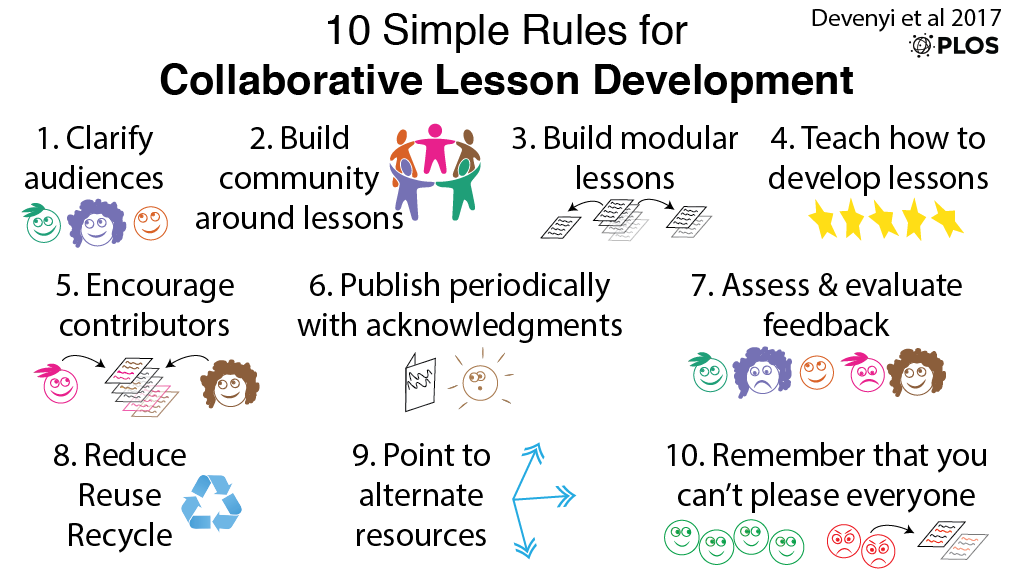
\includegraphics[width=\linewidth]{figure1}
\caption{Graphical abstract of 10 simple rules for collaborative lesson development}
\label{figure1}
\end{figure}
%

\rulemajor{Clarify your audience}

The first requirement for building lessons together is
to know who they are being built for.
``Archaeology students'' is far too vague:
are you and your collaborators thinking of
first-year students who need an introduction to the field,
graduate students who intend to specialize in the sub-discipline which is the lesson's focus,
or someone in between?
Prerequisite knowledge,
equipment or software required,
how much time learners will have:
if different contributors believe different things about these,
they will find it difficult or impossible to work together.

Thinking systematically about difficulty levels can help manage expectations.
For example,
Programming Historian project labels lessons ``beginner'',
``intermediate'',
and ``advanced''
to help authors write at appropriate levels.
This method works, however, only if there is prior agreement on what those terms mean.

Rather than itemizing prior knowledge and learning objectives,
it can be helpful to write \emph{learner profiles} to clarify
the learner's general background,
what they already know,
what \emph{they} think they want to do,
how the material will help them,
and any special needs they might have.

\rulemajor{Build community around lessons}

Lessons do not maintain themselves.
For technical lessons, software versions and dependencies are constantly changing,
while for more traditional academic lessons the literature is advancing at an ever increasing pace.
In either case, what was cutting edge in 2017 may be dated
and less useful in 2018.
This needs to be clear to contributors,
so they understand that this lesson is just
the starting point.
Sustainability needs to be front of mind.

The focus accordingly needs to be on creating a community.
Authors cannot be expected to maintain continual vigilance on a lesson,
but this is necessary if one expects continual use of a lesson!
By working online, creating opportunities for collaboration
and contribution, many eyes can keep the lesson usable.
As we describe in Rule~5,
this only works if you make space for
little contributions just as you do for larger ones.

\rulemajor{Build modular lessons that can be re-purposed}

Every instructor's needs are different,
so build small chunks that can be re-purposed in many ways.
A university lecturer in meteorology, for instance,
might construct a course by bringing together lessons on differential equations,
fluid mechanics and absorption spectroscopy.
This task is greatly simplified if existing courses on mathematics,
physics and chemistry consist of numerous small, discrete lessons,
as opposed to a few large, monolithic lessons.

Doing this shifts the instructor's burden from writing to finding and synthesizing,
both of which are easier if lessons have been designed by people with a shared world-view (Rule~4),
and if lessons clearly signal what they cover (Rule~1).
In particular,
if lessons reference specific points in the model curriculum guidelines promulgated by many professional societies,
it can be much easier for people to find them and integrate them.

Note also that individual lesson topics hinge on the learners having the proper prerequisite background,
so this rule further emphasizes the importance of Rule~1.

\rulemajor{Teach best practices for lesson development}

Decades of pedagogical research has yielded many insights into
how best to build and deliver lessons \cite{hlw}.
Unfortunately,
since most college and university faculty have little or no training in education,
this knowledge and expertise is rarely transferred into classroom practice.

Experience shows that even a brief introduction to a handful of key practices
can help collaborative lesson development in at least three ways.
If people have a shared understanding of how lessons should be developed,
it is easier for them to work together.
Less obviously,
if people have a shared model of how lessons will be \emph{used},
they are more likely to try to build the same kind of material.
Finally,
teaching people how to teach is a great way to introduce them to each other and build community.

An example of a particular lesson development practice is \emph{reverse instructional design}
\cite{wiggins-mctighe}.
When this is used,
lessons are built by
identifying learning objectives,
creating \emph{summative assessments} to determine whether those objectives have been met,
designing \emph{formative assessments} to gauge learners' progress
and give them a chance to practice key skills,
putting those formative assessments in order,
and only then writing lessons to connect each to the next.
This method is effective in its own right,
but its greatest benefit is that it gives everyone a common framework
within which to collaborate.

An example of how to teach these practices is Software Carpentry's instructor training program.
First offered in 2012,
is now a two-day course delivered both in-person and online
\cite{lessons-learned,instructor-training,how-to-teach-programming}.
Not only does it teach good pedagogical practices,
it serves and an introductory process to get everyone on the same page
regarding who lessons are for,
how they are delivered,
and how they are maintained.

\rulemajor{Encourage and empower contributors}

Making the process for contributing to a lesson explicit is
the key to receiving contributions.
New contributors require a straightforward and transparent introduction
to understand the process of tweaking and adapting lessons.
Licensing, code of conduct, governance, and contribution procedure
all need to be explicit rather than implicit
to lower the social barriers to contribution.

Tools can help,
especially if they allow proposed changes to be viewed and discussed
prior to their incorporation into the lessons
(in open source software development this is known as ``pre-merge review'').
Providing a gentle on-ramp for new contributors is essential,
but some tools come with a considerable up-front learning curve.
Housing lessons on GitHub (a web-based version control system)
with changes suggested via pull requests (requests to incorporate changes) is
ideal for pre-merge review, for instance,
but it requires contributors to know how to use Git,
which has a notoriously steep learning curve \cite{git-survey}.
Allowing people to edit a Google Doc or Wiki-based editing does not offer pre-merge review,
but the low barrier to entry can help get conversations started.

The best way to choose tools for managing lessons
is to look for those that provide a gentle on-ramp for new contributors.
Ask potential contributors what they are comfortable with
rather than requiring \emph{them} to come to \emph{you}.
Remember also that contributing to a lesson is probably not their top priority,
and look for ways to reduce their cognitive load.
For example,
threaded discussion on particular topics (e.g., using GitHub issues)
can help increase the signal-to-noise ratio
by reducing long reply-all email exchanges.
Several open frameworks are available to facilitate
development of new lessons, such as R-based
learnr (\url{https://rstudio.github.io/learnr}) or
GitHub-based Morea (\url{https://morea-framework.github.io}) and
DataCamp (\url{https://www.datacamp.com/teach/documentation}).

Finally,
working in the open can be great,
but can also unintentionally suppress voices.
At Programming Historian,
for example,
an ombudsperson is available for private chats and facilitation.

\rulemajor{Publish periodically and recognize contributions}

Like software,
lessons should have releases of fixed content
so that learners or instructors who may wish to use the material have a stable version to refer to
for the duration of their use.
These releases should be periodic
so that improvements and adjustments are made available
for new learners and instructors just starting their use.
Periodic releases are also essential
for enabling recognition of the contribution of authors and maintainers.

Academia has only a few ways of recognizing contributions.
Until these are expanded,
it is important to publish lessons in ways that traditional academic systems can digest.
One is to give particular releases of lessons
DOIs supplied by providers such as Zenodo (\url{https://zenodo.org/})
or DataCite (\url{https://www.datacite.org/}).
Contributors can be listed as authors
and the maintainers of the lesson as editors
to differentiate recognition of their contributions.
Each time the lesson is published,
names and identifiers (e.g. ORCIDs (\url{https://orcid.org}))
should be gathered for all contributors.

A lesson release is a good opportunity to bring the material into a stable shape
by fixing outstanding issues and merging contributions.
Version control helps a lot in continuously maintaining a list of contributors
but also in remembering which version is used for release
(e.g., using branches or tags).
Lesson releases should use a consistent naming scheme,
such as the full year and month of the release,
e.g. ``2017.05''.
This is the scheme Software Carpentry has used in
its releases of its lessons \cite{shell2015,shell2017}.

If lessons are being released regularly,
automate the process.
Old versions of lessons should be archived in a discoverable location for reference.

\rulemajor{Evaluate lessons at several scales}

The purpose of feedback is to guide lesson development
so that authors aren't designing and arguing in a vacuum.
What people immersed in the lessons think needs fixing
can often differ from what learners think.

Micro-scale feedback can be gathered by an instructor while teaching a particular lesson.
Learners might provide feedback on things like typographical errors,
clarity/ease of quiz questions or the order in which topics are presented,
which the instructor can enter into a work-tracking system (e.g., GitHub issues) at the end of class.
As well as encouraging direct verbal feedback,
it's a good idea to provide learners with a means to provide feedback anonymously during class
(e.g., on small pieces of paper like sticky notes).

Pre- and post-class surveys can be used to discover larger macro-scale issues.
These issues often relate to the fact that it can be difficult for lesson developers
to fully understand the frame of reference of their audience.
For instance, a lesson might inadvertently assume prior knowledge that learners do not have,
which is information that can be collected in a survey.
If possible, it's a good idea to conduct the post-class survey 30--60 days after the fact.
This delay allows people time to reflect,
meaning they are more likely to give accurate feedback on what they learned
rather than how entertained they were.

Pre- and post-class surveys also are essential in focusing in on the audience for a given lesson.
Referring back to Rule~1,
it can sometimes be difficult for lesson developers to understand the frame of a given learner,
so surveys (particularly post-class surveys) can reveal hidden assumed knowledge
that can be expanded on or acknowledged to refine the target audience.

\rulemajor{Reduce, re-use, recycle}

Do not create a new lesson if there is an existing one that you can use or contribute to.
Just as a scholar would not write a paper without a literature review,
the same holds for lessons.
Before writing that introduction to the Bash command line,
for example,
do a search:
has anybody else written it?
Is it complementary to your goals?
Could it be tweaked or modified to meet your own goals?
Could your planned lesson be tweaked to compliment the existing lessons so that topics aren't duplicated?

Before re-using content,
make sure to check that the lesson is licensed in an open manner.
Both Programming Historian and the Carpentry projects
use the Creative Commons - Attribution license
(\url{https://creativecommons.org/licenses/by/4.0/}),
which allows people to share and adapt material for any purpose
as long as they cite the original source.

The same questions of re-use come when thinking about recycling content of a lesson,
such as images, data, figure, or code.
Does the license cover that as well?
If not,
then ask permission,
just as you would for any other material.

The converse of this rule is to license your own lessons in a similar open manner,
and to make them discoverable.
For example,
when lessons are published (Rule~6),
make sure that they have the usual keywords in their bibliographic entries
and HTML page headers.

\rulemajor{Link to other resources}

Most learners are unlikely to absorb everything there is to know about a topic
from your lesson alone.
This is partly a matter of scope---any interesting subject is too large
to fit in a single lesson---but also a matter of level and direction.
As Caulfield has argued \cite{choral-explanations},
the best resources provide a chorus of explanations
that offer many angles and approaches for any given topic,
each of which may be the best fit for a different subset of people.

Find these resources and direct learners to them at strategic points.
These resources may include textbooks,
technical documentation,
videos,
and web pages;
if a community or discussion forum exists for the topic,
be sure to include them as well.

Doing this is substantial work,
and maintaining it is even more so,
which makes building community around lessons (Rule~2) all the more important.
In particular,
it is vital to engage the learners as equal participants in that community:
they should both be able to propose updates, corrections, and additions to lessons,
and know that they are encouraged to do so (Rule~5).

\rulemajor{You can't please everyone}

No single lesson can be right for every learner.
Two people with no prior knowledge of a specific subject
may still be able to move at different speeds
because of different levels of general background knowledge.
Similarly,
lessons on ecology for learners in Utah and Florida
will probably be more relatable if they use different examples.
Equally,
no lesson development community can serve all purposes.
Some groups may prioritize rapid evolution,
while others may prefer a ``measure twice, cut once'' approach.

If there are complementary ways to explain something,
or points of view that can cohabit respectfully,
it may be possible to present them side by side.
There are good pedagogical reasons to do this
even if contributors \emph{do not} disagree:
weighing alternatives fosters higher-order thinking,
and as Caulfield has written,
the most popular online question and answer sites
are successful in part because they present a chorus of explanations
geared at different levels and needs
rather than a single one \cite{choral-explanations}.

But sometimes choices must be made.
The open source software community has wrestled with these issues for three decades,
and has evolved some best practices to address them
\cite{producing-oss}.
As discussed in Rule~5,
the first step is to have a clear governance structure and a clear, permissive license.
Minor disagreements should be discussed openly and respectfully.
If they cannot be resolved---i.e., if they turn out not to be so minor after all---then
contributors should split off and evolve the lesson in the way they see best.
(This is one of the reasons to have a permissive license.)

These splits rarely happen in practice.
When they do,
it is important to remember that we all share the same vision of better lessons, built together.

\section*{Conclusion}

Every day,
teachers all over the world spend countless hours duplicating each other's work.
These ten rules provide an alternative:
adopting the model of collaborative software development
to make more robust and sustainable lessons
that can be continually improved by those who use them.
We hope that our experiences can help others teach more
with more impact and less effort.

\nolinenumbers

% Either type in your references using
% \begin{thebibliography}{}
% \bibitem{}
% Text
% \end{thebibliography}
%
% or
%
% Compile your BiBTeX database using our plos2015.bst
% style file and paste the contents of your .bbl file
% here. See http://journals.plos.org/plosone/s/latex for
% step-by-step instructions.

\begin{thebibliography}{1}

\bibitem{hlw}
Ambrose SA, Bridges MW, DiPietro M, Lovett MC, Norman MK.
\newblock How Learning Works.
\newblock Jossey-Bass; 2010.

\bibitem{wiggins-mctighe}
Wiggins G, McTighe J.
\newblock Understanding by Design.
\newblock 2nd ed. Association for Supervision and Curriculum Development; 2005.

\bibitem{lessons-learned}
Wilson G.
\newblock Software Carpentry: Lessons Learned.
\newblock F1000Research. 2016;3(62).
\newblock doi:{10.12688/f1000research.3-62.v2}.

\bibitem{instructor-training}
Christina Koch and Greg Wilson (eds.)
\newblock Software Carpentry: Instructor Training; 2016.
\newblock \url{https://zenodo.org/record/57571#.WS8huDOZPdQ}.

\bibitem{how-to-teach-programming}
Wilson G.
\newblock How to Teach Programming (And Other Things).
\newblock Lulu.com; 2017.

\bibitem{shell2015}
Gabriel A.~Devenyi and Christina Koch (eds.):
Software Carpentry: The Unix Shell; 2015.
\newblock \url{https://zenodo.org/record/27355#.WS8lajOZPdQ}.

\bibitem{shell2017}
Gabriel A.~Devenyi and Ashwin Srinath (eds.):
Software Carpentry: The Unix Shell; 2017.
\newblock \url{https://zenodo.org/record/278226#.WS74tTOZPdQ}.

\bibitem{choral-explanations}
Caulfield M. Choral Explanations; 2016.
\newblock https://hapgood.us/2016/05/13/choral-explanations/.

\bibitem{producing-oss}
Fogel K.
\newblock Producing Open Source Software.
\newblock O'Reilly; 2005.

\bibitem{git-survey}
GitLab
\newblock Global Developer Survey.
\newblock http://get.gitlab.com/global-developer-survey/; 2016.

\end{thebibliography}

\end{document}
